\documentclass[10pt]{article}
\usepackage[usenames]{color} %used for font color
\usepackage[utf8]{inputenc} %useful to type directly diacritic characters
\usepackage{times}
\usepackage[right=3.7cm, left=3.7cm]{geometry}

\usepackage{tikz}                    % for drawing
\usetikzlibrary{positioning}
\usetikzlibrary{shapes}
\usetikzlibrary{arrows}
\usetikzlibrary{calc}
\usetikzlibrary{decorations.pathreplacing}
\usetikzlibrary{backgrounds}

\begin{document}
\begin{figure}[tb]
  \centering
    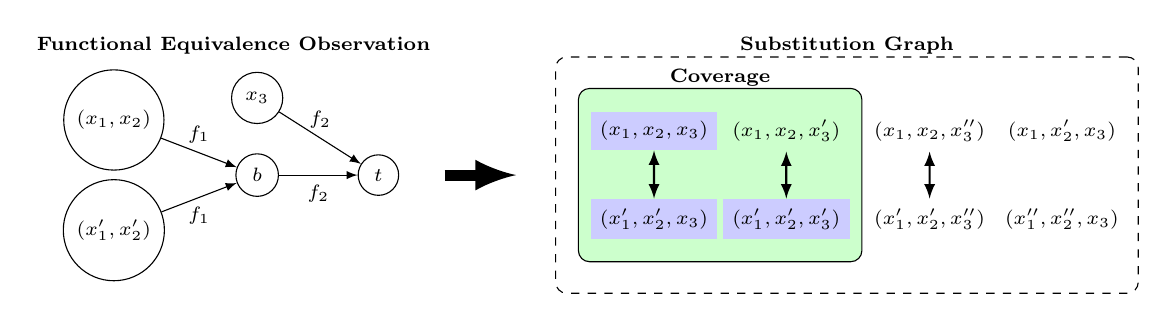
\begin{tikzpicture}[%
        scale=0.7,
        font=\scriptsize,
        node distance=1.4cm,
        %background rectangle/.style={fill=white},
        %show background rectangle,
        >=latex,
    ]
        
        % Style for round nodes (left side)
        \tikzstyle{round} = [draw, circle, minimum size=1em, align=center]
        
        % (e1, e2)
        \node[round] (x1) at (-2,0) {$(x_1, x_2)$};
        
        % (e1', x_2')
        \node[round] (x2) at (-2,-2) {$(x_1', x_2')$};
        
        % Intermediate node b
        \node[round, ] (b) at (0.6,-1) {$b$};
        
        % e3
        \node[round, label={[xshift=-0.3cm,yshift=0.1cm] \textbf{Functional Equivalence Observation}}] (e3) at (0.6,0.4) {${x_3}$};
        
        % Final output t
        \node[round] (t) at (2.8,-1) {$t$};
        
        % Edges: f1 => b
        \draw[->] (x1) -- node[midway,above] {$f_1$} (b);
        \draw[->] (x2) -- node[midway,below] {$f_1$} (b);
        
        % Edges: b, e3 => t
        \draw[->] (b) -- node[midway,below] {$f_2$} (t);
        \draw[->] (e3) to node[midway,above] {$f_2$} (t);

        \draw[->, line width=1.4mm] (4.0,-1) -- (5.3,-1);
 
        \node[draw, rectangle, dashed, rounded  corners, minimum width=7.4cm, minimum height=3cm,
              label={[xshift=0cm,yshift=-0.1cm] \textbf{Substitution Graph}} ] 
              (eqgroup) at (11.3,-1) {};
        
        \node[draw, rectangle, rounded  corners, minimum width=3.6cm, minimum height=2.2cm, 
              label={[xshift=0cm,yshift=-0.1cm] \textbf{Coverage}}, fill=green!20] 
              (eqgroup) at (9,-1) {};
        
        \node[font=\scriptsize, fill=blue!20] (g1) at ($(eqgroup.center)+(-1.2,0.8)$)
               {$(x_1,x_2,x_3)$};
        \node[font=\scriptsize, fill=blue!20] (g2) at ($(eqgroup.center)+(-1.2,-0.8)$)
               {$(x_1',x_2',x_3)$};

        \node[font=\scriptsize] (g3) at ($(eqgroup.center)+(1.2,0.8)$)
               {$(x_1,x_2,x_3')$};
        \node[font=\scriptsize, fill=blue!20] (g4) at ($(eqgroup.center)+(1.2,-0.8)$)
               {$(x_1',x_2',x_3')$};

        \node[font=\scriptsize] (g5) at ($(eqgroup.center)+(3.8,0.8)$)
               {$(x_1,x_2,x_3'')$};
        \node[font=\scriptsize] (g6) at ($(eqgroup.center)+(3.8,-0.8)$)
               {$(x_1',x_2',x_3'')$};

        \node[font=\scriptsize] (g7) at ($(eqgroup.center)+(6.2,0.8)$)
               {$(x_1,x_2',x_3)$};
        \node[font=\scriptsize] (g8) at ($(eqgroup.center)+(6.2,-0.8)$)
               {$(x_1'',x_2'',x_3)$};
        
        \draw[<->, thick] (g1) -- (g2);
        \draw[<->, thick] (g3) -- (g4);
        \draw[<->, thick] (g5) -- (g6);
        
    \end{tikzpicture}
    % \vspace{-2mm}
    \caption{\small
    \textbf{Illustration of functional equivalence.}
    \textbf{Left:} In a two-hop task $(x_1, x_2, x_3) \mapsto t$ with $t=f_2(f_1(x_1,x_2),x_3)$, two fragments $(x_1,x_2)$ and $(x_1',x_2')$ satisfying $f_1(x_1,x_2)=f_1(x_1',x_2')=b$ consistently yield the same final output when combined with the same context $x_3$, supporting their \textbf{functional equivalence}.
    \textbf{Right:} Among all possible inputs (few shown), we draw an edge between any two inputs that differ only by functionally equivalent fragments to form a \textbf{substitution graph}.
    Then, \textbf{coverage} is the set of observed inputs (highlighted as blue) and all inputs connected to them. We define pattern matching as a type of generalization that occurs inside the coverage, harnessing functional equivalence.}
    \label{fig:coverage_illustration}
    % \vspace{-6mm}
\end{figure}
\end{document}